% % !TeX root = ICCPS18.tex
% \subsection{Implementation}

% \begin{figure}
% 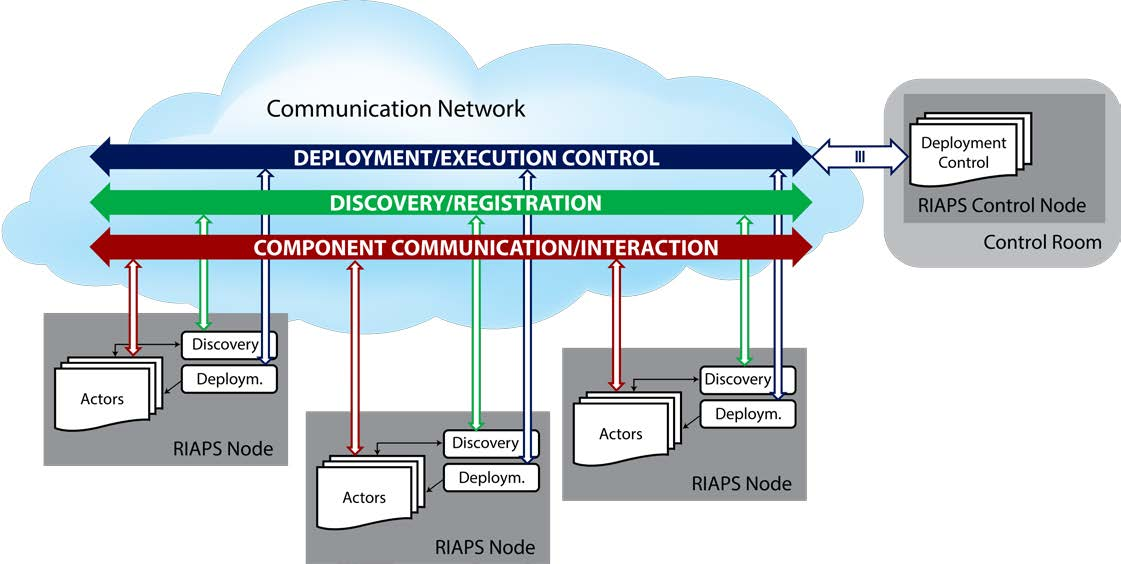
\includegraphics[width=0.48\textwidth]{diagrams/RIAPSBroch_FINALPRINT.jpg}
%   \caption{RIAPS concept.}
% 	\label{fig:concept}
% \end{figure}

% \AronC{This is the only ``subsubsection'' within this subsection.}
% \Abhishek{Aron- the smart contract discussion and the wrapper implementation discussion should go into this section}

% \subsubsection{Background}
% In any technical system that relies on embedded computing, the most important ingredient is an ``operating system'' that provides the foundations for all algorithms, isolates the hardware details from the algorithms, and provides essential mechanisms for resource management, fault tolerance, and security. For example, in the work presented in this paper, this framework allows us to disseminate information between the actors. This platform called `Resilient Information Architecture Platform for Smart Grid' (RIAPS) \cite{riaps} has been developed by our extended team, where each actor is a composition of several libraries that provide (1) a component model that provides a concurrent model of computation for building distributed real-time applications, (2) a messaging framework for facilitating interactions among actors, (3) a resource-management framework for controlling the use of computational resources, (4) a fault-management framework for detecting and mitigating faults in all layers of the system, (5) a security framework to protect the confidentiality, integrity, and availability of system under cyber-attacks, (6) a fault tolerant time synchronization service,  (7) a discovery framework for establishing the network of interacting actors of an application, and (7) a deployment and management framework for the administration and control of the distributed applications from a control room. 


% \subsubsection{Smart Contract}


% \subsubsection{SmartHomeTrader}


% \subsubsection{Solver}


% \Abhishek{Aron we need to describe the implementation architecture.}

% \begin{itemize}
% \item communication is implemented via ZeroMQ
% \item timesynchronization is implemented via PTP and NTP 
% \item Resource discovery if required can be provided by RIAPS. Not required for this experiment.
% \begin{itemize}
% \item The basic implementation pattern is using wrappers to connect to blockchain. Why is this important.
% \item What does the prosumer script do
% \item run one geth client per prosumer
% \item multiple miner nodes can run.
% \item The full architecture includes DSO script, 
% \item Evaluation - Timing and Network Overhead
% \end{itemize}
% \end{itemize}